

%%% This LaTeX source document can be used as the basis for your technical
%%% report. Intentionally stripped and simplified
%%% and commands should be adjusted for your particular paper - title, 
%%% author, citations, equations, etc.
% % Citations/references are in report.bib 

\documentclass[conference,backref=page]{acmsiggraph}

\TOGonlineid{45678}
\TOGvolume{0}
\TOGnumber{0}
\TOGarticleDOI{1111111.2222222}
\TOGprojectURL{}
\TOGvideoURL{}
\TOGdataURL{}
\TOGcodeURL{}

% Include this so that citations show up in blue and the page information is included in the reference section
\hypersetup{
    colorlinks = true, 
    linkcolor = blue,
    anchorcolor = red,
    citecolor = blue, 
    filecolor = red, 
}


\title{Week 1 Game\\
	   Astral Insanity}

\author{Neil Notman, Sam Serrels \\
Edinburgh Napier University\\
Advanced Games Engineering(SET10110)}
\pdfauthor{Neil Notman, Sam Serrels }

\keywords{radiosity, global illumination, constant time}

\begin{document}

\teaser{
   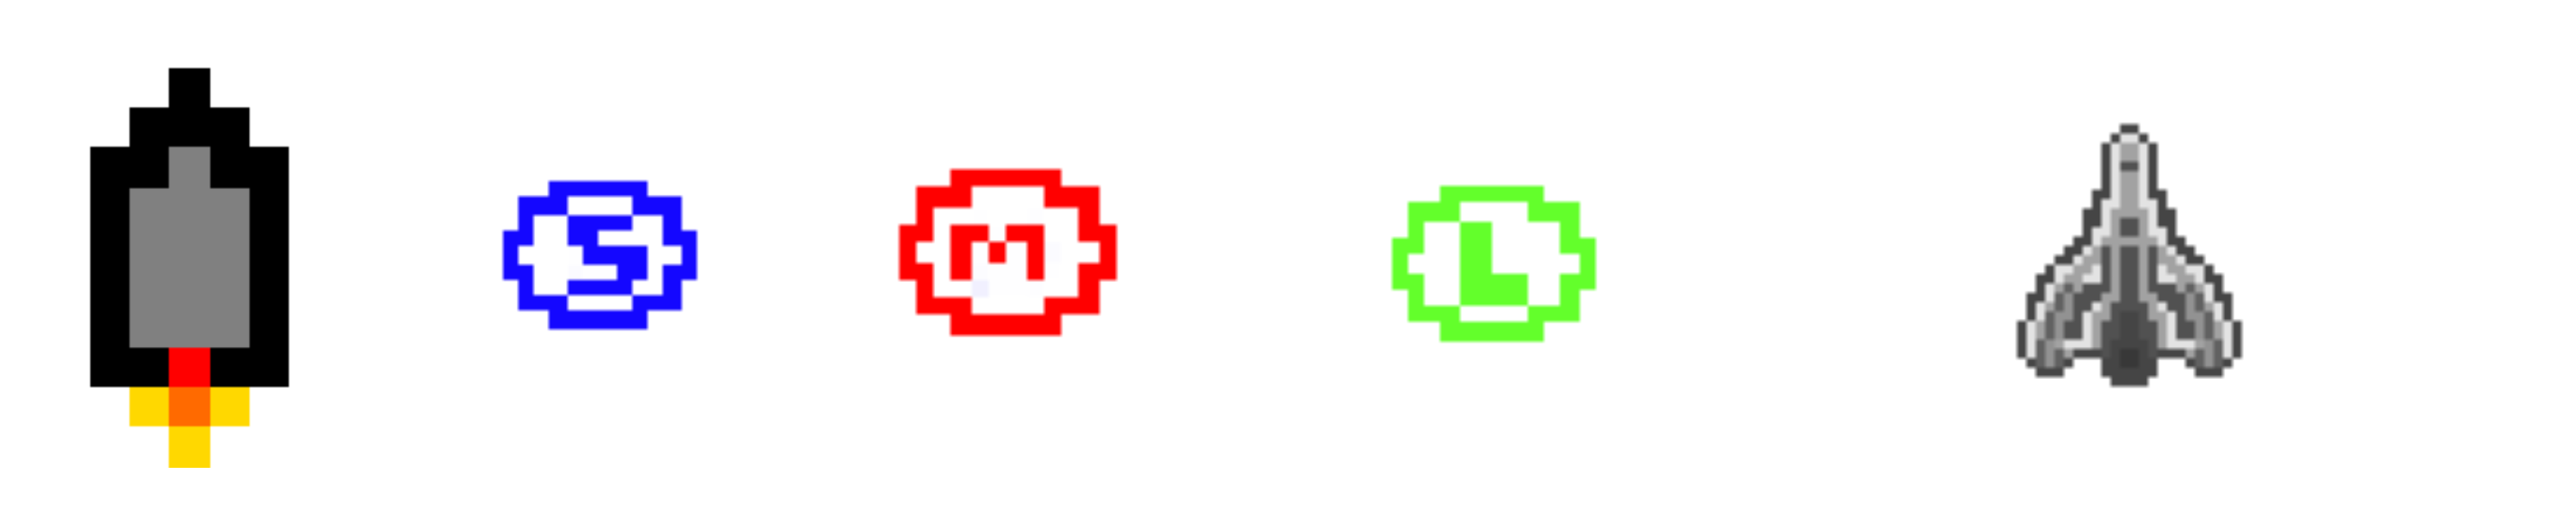
\includegraphics[height=1.5in]{images/sampleteaser}
   \caption{Place a teaser image at the top of your report to show key examples of your work (e.g., multiple screenshots of the different test situations) - Every figure should have a caption and a description.  For example, each figure is labelled and explained: (a) soft bodies, (b) particles, (c) inverse kinematics, (e) fur shells, and (f) position-based dynamics for cloth effects.}
   \label{fig:teaser}
 }

\maketitle

\begin{abstract}

The abstract is typically a single paragraph.  The abstract is the first thing people read when they encounter your report; hence, it is crucial that it outlines all the important aspects of your report.  Make your abstract incredibly concise and clear.  You start with the problem and end with why your solution is interesting.  Briefly explain why your solution is valuable and how you have evaluated it.  Keep your abstract small.  Typically, the abstract should be approximately 100 words.

\end{abstract}



\keywordlist

%% Use this only if you're preparing a technical paper to be published in the 
%% ACM 'Transactions on Graphics' journal.

% \TOGlinkslist

% \copyrightspace


\section{Introduction}

The introduction sells your physics-based simulation effect.  It tells the reader about the problems and motivation.  It tells the reader about why it is important.  Your introduction should be five clear well defined paragraphs \cite{day2012write}.

\begin{itemize}
\item What problem are you solving?
\item What is the motivation? (What's so interesting and important?)
\item Why is it hard? (e.g., why do naive approaches fail?)
\item Why hasn't it been solved before or what are you doing differently? How does yours differ?
\item What's your approach?  How will you solve the problem?  Are their any specific limitations?
\item (Optional) How the rest of the report is structured.\\
e.g., The rest of this report is structured as follows: first we discuss the related work in section 2, and then describes the implementation in Section 3.  Section 4 describes how we intent to evaluated our system.  Section 5 gives the conclusions.
\end{itemize}

\paragraph{Starting examples:}
This report attempts to addresses the problem of the applicability of …. in ….. by considering …...  It surveys a number of answers to this question.  Our method offers a simplistic, robust, and reliable scheme.

This report attempts to introduce the reader to …… 
(Catch the readers attention, Anecdotes, Proverbs, Facts, Real-World Examples...)

The problem this report address is …..


\section{Related Work}

Refer to literature on the particular physics-based animation effect you want to synthesize (e.g., published articles, books, conference proceedings, web articles) provide a comprehensive review - and use the correct citation format, e.g., \cite{Sako00}.

Related work should finish with a summary paragraph - emphasising the crucial similarities or differences between existing methods presented in the literature.  For example: (1) you might want to modify the technique to run on the GPU; (2) or you combine different techniques from different authors; (3) or you are simplifying the algorithm to make it run faster.

\section{Overview}
Brief overview of the core principles and mechanism behind your effect.  This should be reflected in your final implementation, so consider what you will actually be implementing. What components make up the effect and how are they connected.


\section{Simulation}

How does your simulation work and what are the reasons it is important.  This is a decisive section to put together as it will help you in the rest of your physics-based animation development.

\begin{itemize}
\item{Physics-Based Animation Description}
Provide a more detailed description of how the simulation functions.
\item{Formal Elements}
Description of your simulation using the formal elements.  You should include the following sections.
\item{Interactive}
Describe the interactive pattern you are aiming for .
\item{Objectives}
What are the objectives of the simulation?  You may have one overall objective and some sub-objectives.
\item{Procedures}
What are the actions performed in the simulation.  Are there any specific technical workings?
\item{Rules}
What test cases have you defined to demonstrate the effectiveness of your technique?  Define a list of simple tests - both showing the good and the bad parts of your approach.
\item{Resources}
What are the resources within the solution?  Is it procedural?  Does it require artist intervention?  Is the solution scalable?  e.g., large and small scenes?
\item{Boundaries}
What are the boundaries of the technique?  This will probably be based on experiments - the technique might only fit specific situations (e.g., outside/inside/small high detail situations or crowds of low-level detail).
\item{Outcome}
What is the outcome?  Explain any possible issues?  Complexity? Computational power? Remember, relate this back to your investigations, related work, and experience - what have other people said?  Do you agree with them?
\end{itemize}

\section{Description}

\begin{itemize}
\item {Screen Mock-Ups \& Preliminary Screenshots}
Provide any screen mock-up of how your animation will look or preliminary screenshots.  You can use whatever method you see fit to create the mock-up.  Your mock-up doesn't have to be exactly how your simulation will look, and you can use in place graphics.  Explain principles and concepts to the reader - so you can explain your idea.
\item {Dynamic}
In this section you should describe any user interactive controls for customizing or changing the simulation - to effect the outcomes of the effect (e.g., adding external forces, numbers of objects, gravity)
\item {Control Mechanism}
Describe the control principles.  What controller mechanism have you gone for (i.e., random or from scripts)?  
\item {Rules}
Reflect upon the rules defined in the formal elements, and how these may affect the controls of the simulation.  Also consider any relationships between physical objects which might have an influence on the controls.
\item {Modes and Other Features}
Does your effect support multiple modes?  Are there any other features (e.g. novel control mechanisms) which need to be taken into account?
\item {Test Scenes}
Does your simulation have different scenes (2D, 3D, different complexity, real-time, off-line)?  If so, then design a variety of simple test cases to show the situations and demonstrate the viability of your technique.
\item {Flowchart}
Create an overview flowchart - and explain the interaction of the different components.  For example, do you update the forces, then move forwards, then draw....
\end{itemize}

\section{Technical Specification}

In this section, you should put together some of the technical details of your simulation.  This will help when developing your physics-based simulation later.

\begin{itemize}
\item {Technical Analysis} This section analyses the technical requirements of your simulation.  The goal here is to describe the main software development tasks, the risks involved, and any external libraries you are using.
\item {Major Software Development Tasks} What are the major pieces of development to make the software work?  Identify the main tasks from the simulation design, particularly items you feel will be difficult to implement.  List these here so you can approach these tasks individually.
\item {Risks} What are the risks in your development?  Consider which pieces of functionality will be difficult to implement, and what are the options if you cannot achieve them.
\item {External Libraries} Are you using any external libraries or resources to implement your simulation?  If you are using any libraries outside the ones developed in the practical sessions, these will need to be described here.
\end{itemize}


Equations should be numbered and in the correct format, e.g., Equation \ref{eq:myequation} below:

\begin{equation} \label{eq:myequation}
 \sum_{j=1}^{z} j = \frac{z(z+1)}{2}
\end{equation}

Furthermore, if you include an equation, ensure you explain what each of the variables are (e.g., $F$ is force, $m$ is mass, and $a$ is the acceleration).

\subsection{Common Mistakes}
A list of common mistakes you should avoid:
\begin{enumerate}
\item Don't using 'I' or 'Me'
\item Each paragraph should be clear and focuses with multiple sentences that help make your point - avoid lots of single line paragraph sentence
\item Make sure the citations are done using the correct formatting (i.e., .bib file and let LaTeX generate the references)
\item Every figure should have a caption, explaining what the picture is and what the reader should be looking at (i.e., what is important about the figure, what does it show)
\item A figure should also be referenced in the body of the main text (e.g., see Figure \ref{fig:teaser})
\item Equations should be numbered, and referenced in the text. Furthermore, ensure each of the variables in the equation are explained (i.e., don't use F=ma and not say what F, a, and m are)
\end{enumerate}





\section{Conclusion}
The report should finish with a summary to give a brief overview of what the reader should remember most.  What was most important?


% \section*{Acknowledgements}


\bibliographystyle{acmsiggraph}
\bibliography{report}

\end{document}

